% \section[Probability Weighting]{What are weighting for? A mechanistic explanation of probability weighting}
\section{Main Result}

\begin{frame}{Main results}
\begin{center}
	\includegraphics[width=.9\textwidth]{../../figs/Our_result_LocScale_vs_KT.pdf}
\end{center}
\begin{enumerate}
	\item	generic inverse-S shape can be explained by difference in uncertainty
	\item process of estimation of this uncertainty generates inverse-S shape
% 	\item	relative estimation error in $p(x)$ is greater for rarer events 	
\end{enumerate}
\label{MainResults}
\hyperlink{weight_vs_estimate}{\beamergotobutton{PW K\&T 1979}}
\end{frame}

\section{Probability Weighting}

\begin{frame}{Defining Probability Weighting (PW)}

\begin{columns}[T]
\column{0.5\textwidth}
% \begin{center}
	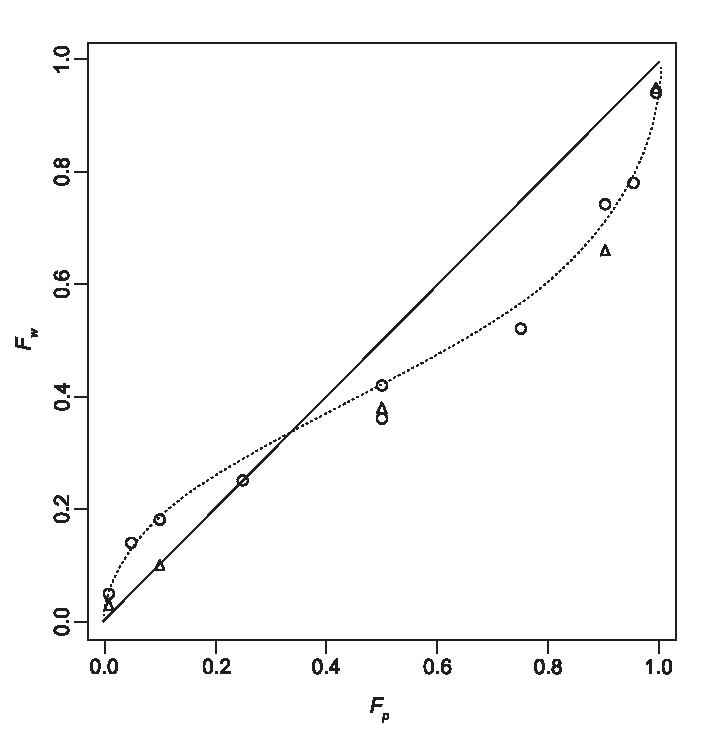
\includegraphics[width=.9\textwidth]{../../figs/TK1992.pdf}
% \end{center}

\parencite[p. 310, Fig. 1,relabelled axes]{TverskyKahneman1992}

\column{0.5\textwidth}
\begin{itemize}
  \item overestimation of rare events $\rightarrow$ underestimation of common events
  \item stable empirical pattern: inverse-S shape
\end{itemize}

\red{Received wisdom:}
\bi
	\item	\red{PW = maladaptive irrational cognitive bias}
\ei

\begin{block}{In search of a mechanism}
	\begin{itemize}
	  \item[$\hookrightarrow$] How does this pattern emerge?
  	\item[$\hookrightarrow$] Can we derive the functional form (rather than merely fitting some function)?
	\end{itemize}
\end{block}

\end{columns}
\end{frame}

\begin{frame}{Set up : A Thought Experiment}
\begin{columns}[T]
\column{0.5\textwidth}
	\centering
	\textbf{Disinterested Observer (DO)} \\
	\vspace{0.5em}
	\includegraphics[height=3cm]{img/TverskyKahnemanFunny} \\
	\vspace{0.5em}
\column{0.5\textwidth}
	\centering
	\textbf{Decision Maker (DM)} \\
	\vspace{0.5em}
	\includegraphics[height=3cm]{img/LabRat} \\
	\vspace{0.5em}
\end{columns}

\begin{columns}[T]
\column{0.05\textwidth}
\column{0.35\textwidth}
	\vspace{0.5em}
% 	\centering
	DO has a \red{model} of the random variable $X$, \eg payout of a gamble \\
	\red{probabilities $p(x)$} \\
  \red{CDF $F_p(x)$}\\
\column{0.2\textwidth}
\centering
	\includegraphics[height=3cm]{img/coinflip}
\column{0.4\textwidth}
	\vspace{0.5em}
% 	\centering
  DM has a \blue{different model} of the same random variable $X$ with greater uncertainty\\
   \blue{decision weights $w(x)$} \\
   \blue{CDF $F_w(x)$}
\end{columns}
\end{frame}

% \section{Location and Scale of PDFs}
% \hyperlink{t-distribution}{\beamergotobutton{HTD}}
% Transmission of different uncertainties from PDFs into CDFs}

\begin{frame}{Types of Different Uncertainties}
\centering
	\includegraphics[width=0.8\textwidth]{../../figs/2GaussianPDFs2Scales2Locations.pdf}
	\includegraphics[width=0.4\textwidth]{../../figs/pdfs_diff_scale_and_loc.pdf}
\end{frame}

% \begin{frame}{The Simplest Case : Different Scales}
% Numerically, our procedure can be applied to arbitrary distributions:
% \begin{enumerate}
% 	\item construct a list of values for the CDF assumed by the DO, \red{$F_p(x)$}
% 	\item construct a list of values for the CDF assumed by the DM, \blue{$F_w(x)$}
% 	\item plot \blue{$F_w(x)$} \vs \red{$F_p(x)$}
% \end{enumerate}
% \vspace{2em}
% \end{frame}

\begin{frame}{The Simplest Case : Different Scales}
\centering
\begin{columns}[T]
\column{0.24\textwidth}
\centering
	\includegraphics[width=1.1\textwidth]{../../figs/2GaussianPDFs2Scales.pdf}
\column{0.76\textwidth}
Numerical procedure applies to arbitrary distributions:
\begin{enumerate}
	\item construct a list of values for the CDF assumed by the DO, \red{$F_p(x)$}
	\item construct a list of values for the CDF assumed by the DM, \blue{$F_w(x)$}
	\item plot \blue{$F_w(x)$} \vs \red{$F_p(x)$}
\end{enumerate}
\end{columns}
\vspace{1em}
\pause
	\includegraphics[width=.9\textwidth]{../../figs/mapping_cdfs.pdf}
\end{frame}

\begin{frame}{Applying the Procedure to the Uncertainty Types}
\centering
	\includegraphics[width=0.75\textwidth]{../../figs/Gauss_scale_location_both_KT.pdf}
	\label{LocationScale}
\end{frame}

\begin{frame}{Interim conclusion}
\bi
	\item greater scale reproduces inverse-S shape
	\item differences in location and scale reproduce asymmetric inverse-S shape
	\item inverse-S shape arises for all unimodal distributions
	\item Probability Weighting is the effect of a difference in uncertainty
	\item[]
	\item[] \textit{Job done. Thank you for your attention ;)}
	\hfill
	\hyperlink{FunctionalForms}{\beamergotobutton{Functional Forms}}
	\label{InterimConclusion}
\ei
	\vspace{2em}
	\centering
	\includegraphics[width=0.8\textwidth]{../../figs/Our_result_LocScale_vs_KT.pdf}
\end{frame}

\section{Ergodicity Question}

\begin{frame}{Asking the Ergodicity Question}
\begin{columns}[T]
\column{.35\textwidth}
	\bc \textbf{DO's concern} \ec
	What happens on average to the \red{ensemble} of subjects?
\column{.02\textwidth}
\centering \vspace{4em}  \red{\large $\neq$}
\column{.49\textwidth}
	\bc \textbf{DM's concern} \ec
	What happens to me \blue{on average over finite time}?
% 	\begin{itemize}
% 	  \item DM's adaptive/ecological rationality $\equiv$ survival, \ie evolutionary incentive to err on the side of caution
% 	  \item[$\rightarrow$] add more uncertainty to his model
% 	\end{itemize}
\end{columns}
\end{frame}


\section{Estimation}
\begin{frame}[allowframebreaks]{Extra Uncertainty is Part of DM's Inference Problem}

DM's adaptive rationality: err on the side of caution:
\begin{itemize}
  \item DM has no control over the experiment,
	\item DM's incomplete comprehension of the experiment/decision problem,
	\item DM needs to trust the DO
	\item uncertain outcome is consequential only to the DM,
% 	\item DM's ignorance,
	\item \ldots
\end{itemize}

\framebreak

% DM's extra uncertainty in the random variable $X$:
\begin{itemize}
	\item ``probability'' is polysemous \quelle{\parencite{Gigerenzer1991,Gigerenzer2018,HertwigGigerenzer1999}}
  \item probabilities are not observable, but
  \item DM observes counts of (rare) events along his life trajectory through time
  \item[$\hookrightarrow$] \textbf{DM's inference problem:} estimate probability $p(x)$ from counts
\end{itemize}
\end{frame}


\begin{frame}{Nature of Inference for Rare Events}
\begin{columns}[T]
\column{0.5\textwidth}
\textbf{Rare Event} %\hfill \includegraphics[height=1.5cm]{img/BlackSwan} \hfill
\begin{itemize}
  \item $p(x) = 0.0001$
  \item 10000 observations
  \item $\sim 99.5\%$ of such time series will contain 0 or 1 events
  \item Na\"ive estimation: $\phat(x) = 0$ or $\phat(x)=0.0001$
  \item[$\hookrightarrow$] either impossible or ten times (over)estimation
\end{itemize}
\column{0.5\textwidth}
\textbf{Common Event} %\hfill \includegraphics[height=1.5cm]{img/WhiteSwan}  \hfill
\begin{itemize}
  \item $p(x)=0.1$
  \item 10000 observations
  \item $\sim 99.5\%$ of time series would contain between 50 and 150 events,
  \item[]
  \item[]
  \item[$\hookrightarrow$] much smaller relative error in $\phat(x)$
\end{itemize}
\end{columns}
\vspace{2em}
% \centering
$\hookrightarrow$ the smaller $p(x)$ the smaller the count of it in a finite time series \\
$\hookrightarrow$ the bigger the relative estimation error
\end{frame}

\begin{frame}{Relative Estimation Error is Larger for Rarer Events}

\begin{center}
\begin{table}[!htb]
  \begin{tabular}{@{}ccccc@{}}
\toprule[2pt]
\makecell{Asymptotic\\probability} & \makecell{Most likely\\count} & \makecell{Standard error\\in count} & \makecell{Standard error\\in probability} & \makecell{Relative error\\in probability}\\
\midrule[2pt]
% .5 &	5000 & 71	& 0.01 & 0.71\%\\
0.1 & 1000 & 32 & 0.003 & 3\%\\
0.01 & 100 & 10 & 0.001 & 10\%\\
0.001 & 10 & 3 & 0.0003& 30\%\\
0.0001 & 1 & 1 & 0.0001 &100\%\\
\bottomrule[2pt]
\end{tabular}
\caption{$T = \num{10000}$, assuming Poisson statistics, relative estimation errors $\sim \nicefrac{1}{\sqrt{\text{count}}}$}
\label{errors}
\end{table}
\end{center}
\end{frame}

\begin{frame}{Estimation of the decision weights}

	Using the count $n(x)$ to form the best estimate and add to it the uncertainty about best estimate 
	\begin{align}
		w(x)						&\approx	\frac{n(x)}{T\delta x} \pm \frac{\sqrt{n(x)}}{T \delta x} \\
		w(x)						&\approx	\phat(x) \pm \err{\phat(x)} 	\elabel{prob_est}
	\end{align}
	with the standard error expressed in terms of the estimate itself
	\begin{align}
		\err{\phat(x)}	&\equiv		\frac{\sqrt{n(x)}}{T \delta x} = \sqrt{\frac{\phat(x)}{T \delta x}} \\
		\lim_{T\to\infty} w(x)	&\to p(x)					
	\end{align}

\end{frame}

\begin{frame}
\begin{center}
  \includegraphics[width=.8\textwidth]{../../figs/dm_count_sim}
\end{center}
\end{frame}

\begin{frame}
\begin{center}
	\includegraphics[width=.8\textwidth]{../../figs/square_root_error}
\end{center}

\end{frame}

% \begin{frame}{Simulation of the Estimation}
% \begin{center}
% 	\includegraphics[width=.65\textwidth]{img/dm_count_sim} \\
% 	$T = 100$, estimates of \red{$\phat(x)$} in red, estimates with one standard error \blue{$\phat(x) + \err{\phat(x)}$} in blue 
% \end{center}
% 
% \end{frame}
% 
% \begin{frame}
% 	Using the fact that $n(x)$ is a random variable itself, $n(x) \sim Poisson$, its fluctuations scale like $\sqrt{n(x)}$ \\
% 
% 	Using the count $n(x)$ to infer the asymptotic PDF as
% 	\begin{align}	  
% 		p(x)	&\approx \frac{n(x)}{T\delta x} \pm \frac{\sqrt{n(x)}}{T \delta x} \\
% 					&\approx \phat(x) \pm \err{\phat(x)}
% 	\elabel{prob_est}
% 	\end{align}
% 	with the standard error (expressed in terms of the estimate itself)
% 	$$\err{\phat(x)} \equiv \frac{\sqrt{n(x)}}{T \delta x} = \sqrt{\frac{\phat(x)}{T \delta x}}$$
% 	\bi
% 		\item standard error $\err{\phat(x)}$ shrinks as the probability decreases
% 		\item relative error in the estimate is $1/\sqrt{\phat(x)T\delta x}$ grows as the event becomes rarer
% 		\item consistent with our claim, that low probabilities come with larger relative errors
% 		\item[$\hookrightarrow$] Errors in probability estimates behave differently for low probabilities than for high probabilities: absolute errors are smaller for lower probabilities, but relative errors are larger
% 	\ei
% \end{frame}

\section{Conclusion}

\begin{frame}{Conclusion}
\lmlblue{Ergodicity Economics explains probability weighting}
\begin{itemize}
  \item inverse-S shape as a neutral indicator of a difference in opinion
%   \item relative probability estimation errors are greater for rarer events
	\item reported observations are consistent with DM's extra uncertainty
	\item relative uncertainty arises out of the situation of the DM over time
	\item reproduce the right type of uncertainty, \ie relative errors are larger for rare events
  \item[$\hookrightarrow$] Probability weighting is rational cautious behaviour under uncertainty over time
  \item[]
  \item See full paper at \url{bit.ly/lml-pw-r1}
  \item links to play with the code are inside
%   \\ \fullcite{PetersETAL2020R1}
% 	\item See blog post for the basic reasoning \fullcite{Peters2020}
% 	\item See blog post for the basic reasoning \fullcite{Buchanan2020}
\end{itemize}

\end{frame}
